\chapter{Results and Discussion} \label{chap_results}

This chapter will present the results from performance testing our purposed architecture. Section \ref{sec_results} will present the setup to our experiments and their respective results, while Section \ref{sec_discussion} will provide our analysis of the results. 

\section{Results} \label{sec_results}

\subsection{Hardware Resources}

The architecture described in Chapter \ref{chap_method} was prototyped on an \textit{Avnet Zedboard}, containing a \textit{Xilinx Zyngq-7020 All Programmable System-On-Chip} (SoC). The SoC contains two ARM Cortex-A9 processors, and a Artix-7 FPGA. 

The main reason for choosing this system was that it contains four DMA channels, and 220 DSP slices, which should have allowed us to run four fully saturated accelerators in parallel. Unfortunately resource constraint for our architecture turned out to be \textit{look-up tables} (LUTs)

In this prototype we were only able to use one of the two ARM processors for controlling the accelerator(s) and processing the layers that were not accelerated. Preferably we should have used both for processing layer C5 and F6, but we were unable to do so due to time constraints. 

(Not done yet, will add more information on what hardware resources on the FPGA was used, and how this changes when adding more accelerators). 


\subsection{Performance}

In order to determine the execution speed and power efficiency of our system we have compared it to the ARM Cortex-A9 CPU on the Zedboard and an ASUS X550JK laptop with a Intel Core i7 4710HQ CPU. Both CPUs ran the pure software implementation of the CNN, while our system used a combination of hardware and software, as described in \ref{chap_method}. We ran our own system with three different configurations:

\begin{itemize}
	\item Accelerating layer C1 and S2. 
	\item Accelerating layer C1, S2, C3 and S4.
	\item Accelerating layer C1, S2, C3 and S4. In addition, the input images was preprocessed from 32-bit floating point to Q16:16 fixed point. Thus the input to the accelerator does not have to be converted during execution.
\end{itemize}

In order to determine the energy efficiency of the different systems we used the metric \textit{images/Watt}, i.e. number of images processed per Watt. Note that these images are $ 32 \times 32 $, and thus processing one image corresponds to 331104 multiply-and-accumulate operations. We also included a metric for measuring execution speed, using images/second. Despite power efficiency being the main focus of this assignment, execution speed can be interesting for several applications and is closely related to power usage. 

The measurements were done by timing the processing of 10 000 images from the MNIST dataset, while measuring the power consumption. 

Total board power was determined by measuring over pin 1 and 2 on J21 on the Zedboard during execution. With the FPGA programmed and the accelerator activated the board measured to 4.68 W, while the ARM processor alone measured to 4.32 W. We were unable to measure the power consumption of the laptop directly, and therefore used the power estimation provided by ASUS, being 120 W \cite{ASUS2015}.  

The results can be seen in Figure \ref{fig_results_all_layers}.

\begin{figure}[h!]
	\centering
	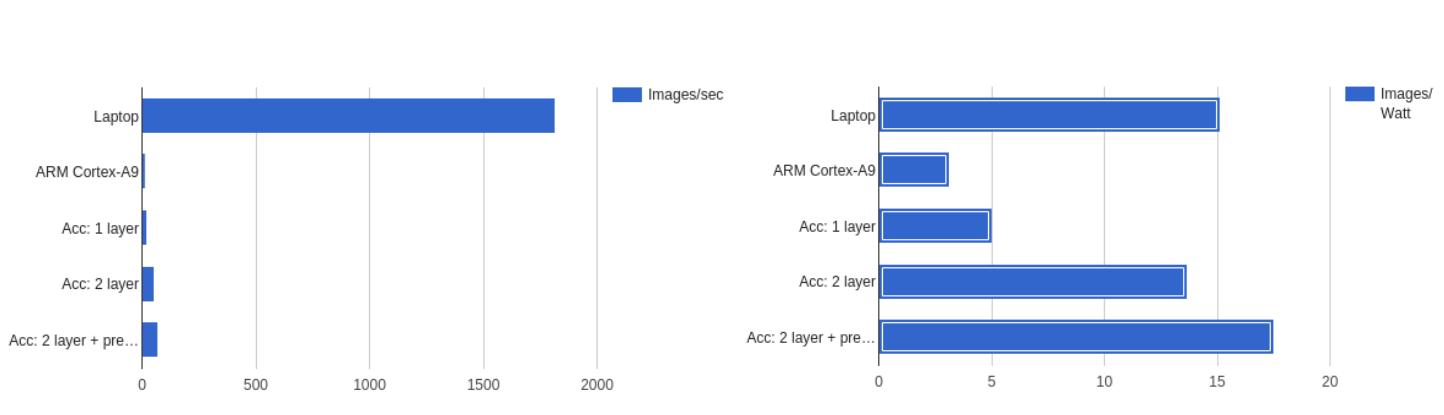
\includegraphics[width=1.0\textwidth]{Figures/Results/results_all_layers}
	\caption{The execution speed and power efficiency measured in number of images processed.}
	\label{fig_results_all_layers}
\end{figure}

We also decided to perform the same measurements when processing only the layers we have hardware accelerated, i.e. C1, S2, C3 and S4. This allowed us to compare the accelerator's performance more directly against the pure software implementations, since layer C5 and F6 shows to be the major bottleneck when processed on the ARM processor. The results are shown in Figure \ref{fig_results_accelerated_layers}.


\begin{figure}[h!]
	\centering
	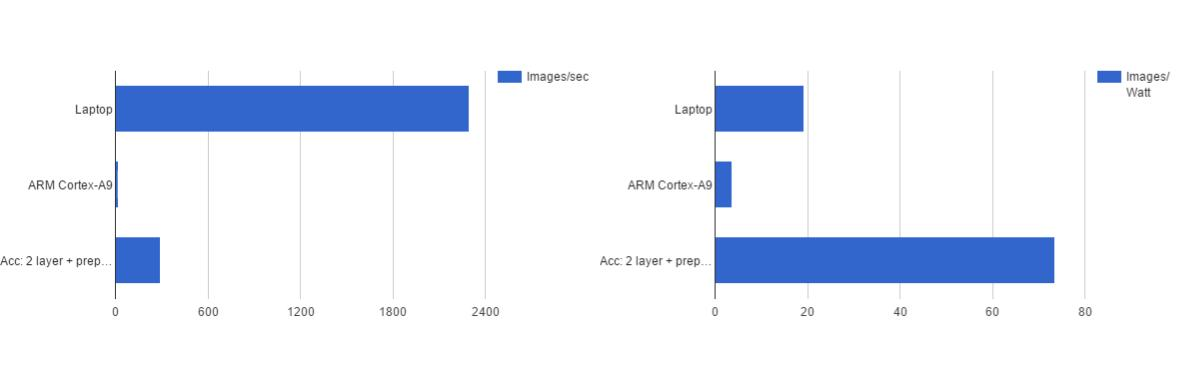
\includegraphics[width=1.0\textwidth]{Figures/Results/results_accelerated_layers}
	\caption{The execution speed and power efficiency measured in number of images processed.}
	\label{fig_results_accelerated_layers}
\end{figure}

\section{Discussion} \label{sec_discussion}

\subsection{Hardware Resources}

\subsection{Performance} 

As can be seen from the Figure \ref{fig_results_all_layers} the accelerator provides a significant boost to both execution and power performance compared to the ARM processor. Accelerating layer C1 and S2 provides a 1.6x speedup, while accelerating C1, S2, C3 and S4 provides a 4.3x speedup. Which is interesting since both layers computes about the same amount of connections (see Table \ref{tab_nofOps}), so why is the ARM processor able to compute C1 faster than C3? We deem that the most probable reason is the cache and memory accesses. In layer C1 the input image can be loaded into cache once and stay there for the duration of the processing of the layer. While in layer C3 there is a set of different input maps and kernels that is required to compute a single output map, thus reducing the ARM processors ability to utilize the cache. 

Figure \ref{fig_results_accelerated_layers} shows the performance when executing the layers that we have accelerated. Here we clearly see how much the accelerator outshines the ARM processor, with a 21x speedup. This also shows that the current bottleneck is now layer C5 and F6. In Section \ref{sec_what_to_accelerate} we deemed unlikely to be worth it to accelerate C5, but these results actually make a strong case for it. 

Compared to the ASUS X550JK our architecture is currently a lot slower, i.e. 26x slower. This is expected, since the laptop contains a state of the art CPU which is highly optimized for execution performance by Intel, while our accelerator is only a prototype. In addition, this network is relatively small compared to the ones described in Chapter \ref{chap_related_work}, consequently leading to less parallelism to exploit. In addition when the input maps become to large to fit into cache, it is likely that the laptop's performance will drop. Thus with larger networks we predict that the difference between the execution time will decrease.

But while our accelerator performs worse in terms of execution speed it performs better in regard to power efficiency in some areas. When running all the layers, our system achieves 15.2 images/Watt while the laptop achieves 15.1 images/Watt, i.e. practice the same. But if we look at only the layers accelerated we see that our accelerator is 3x as power efficient. Based on this we believe that our system will outperform the CPU if the features mentioned in Chapter \ref{chap_related_work} are implemented.  
